\documentclass[/home/greg/Thesis/main/main.tex]{subfiles}

%\title{Neutron star mechanics in the observers inertial frame}
%\author{}

\begin{document}
\graphicspath{{/home/greg/Neutron_star_modelling/TimingNoiseModels/IntroductionToPhysicalObservables/img/}}

\newcommand{\Jr}{\mathbf{J}_{\textrm{rot}}}
\newcommand{\Ji}{\mathbf{J}_{\textrm{in}}}

\section{Definitions}
In chapter \ref{sec: neutron star dynamics in the rotating frame} we
numerically solved Euler's rigid body equations in the rotating body frame
yielding the evolution of the spin vector $\spin$; this allowed us to observe
the dynamics such as precession and alignment without resolving individual
rotations. Physical observations of the star are made in the inertial frame and
so observers report on quantities calculable from the TOA of pulses. Generating
timing models for the phase, they quote results such as timing residuals and
the pulsation frequency and spindown. We aim to simulate these physical
observables and test the effect of timing noise mechanisms. To do
this, we need to transform the solutions of Euler's rigid body equations into
observable quantities in the inertial frame. An efficient way to do this is to
determine the Euler angles which transform the rotating body frame axis,
denoted by $(x',y', z')$, to the inertial frame axis for which we will use $(x,
y, z)$. We will use the Euler angle parameterisation as described by
\citet{Landau1969}; a schematic of how these angles are constructed is given in
figure \ref{fig: Euler}. 
\begin{figure}[ht]
\centering
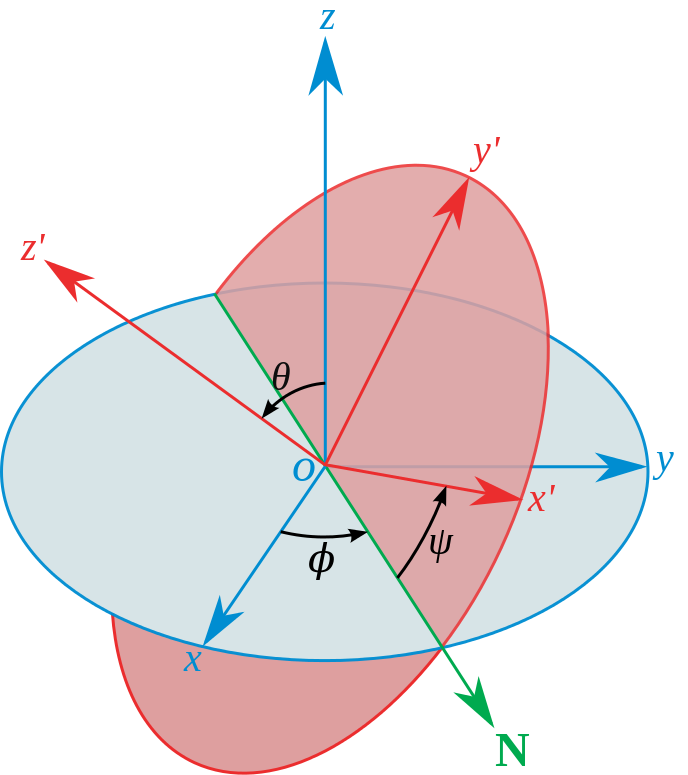
\includegraphics[scale=0.25]{/home/greg/Neutron_star_modelling/Illustrations/EulerAngles/Eulerangles-alternative_filled.png}
% http://commons.wikimedia.org/wiki/File:Eulerangles-alternative.svg
\caption{Schematic of the Euler angle rotation. In the inertial frame the
angular momentum is set to lie initially along the $z$ axis. In the rotating
body frame for a biaxial body the deformation lies along $z'$ while the spin
vector initially lies along in the $x'- z'$ plane.}
\label{fig: Euler}
\end{figure}•

In the body frame, the diagonal moment of inertia tensor has components
$I_{xx}$, $I_{yy}$ and $I_{zz}$ and the star is spun down by a torque
$\boldsymbol{T}$. The Euler rigid body equations are then the left hand side
set of equations in \eqref{eqn: ODEs}. Decomposing the motion of the spin
vector into Euler angles and rearranging yields the right hand set of equations
in \eqref{eqn: ODEs}. These describe the evolution of the three Euler angles.
\begin{align*}
\dot{\omega_{x}} & = \frac{1}{I_{xx}}\left[T_{x} + 
                      \left(I_{yy} - I_{zz}\right) \omega_{y} \omega_{z}\right] 
& 
\dot{\theta} & = \omega_{x} \cos \psi - \omega_{y} \sin \psi
\\
\dot{\omega_{y}} & = \frac{1}{I_{yy}}\left[T_{y} + 
                      \left(I_{zz} - I_{xx}\right) \omega_{x} \omega_{z}\right] 
& 
\dot{\phi} & = \frac{\omega_{x} \sin \psi + \omega_{y} \cos \psi}{\sin \theta}
\numberthis \label{eqn: ODEs}
\\
\dot{\omega_{z}} & =\frac{1}{I_{zz}}\left[T_{z} + 
                      \left(I_{xx} - I_{yy}\right) \omega_{x} \omega_{y}\right]
& 
\dot{\psi} & = \omega_{z} - \dot{\phi} \cos \theta.
\end{align*}

These equations can be solved numerically using a time stepper, for now
we will use the \texttt{rkf45} stepper provided by GSL. % Need reference
%The rotation period of the star is several orders of magnitude smaller than the
%precession period, as a result the Euler angles evolve on a much shorter time
%scale than the body frame spin components. This is numerically expensive. To
%allow efficient investigations we will therefore consider unrealistic values to
%understand the different types of motion before using realistic values only in
%cases of interest.

%Initially only torque free biaxial bodies are considered for simplicity, this
%system was studied by \citet{Jones2001} where it was demonstrated that for a
%biaxial body with deformation $\n_{d}$ along the $z'$ axis, this deformation,
%the spin vector and the angular momentum $\J$ are coplanar. They form a system
%which undergoes two different rotations: firstly at approximately the fast spin
%frequency the system rotates about $\J$ corresponding to a linear increase in
%$\phi$, then at the slower precession frequency the system counter rotates
%about $\n_{d}$ corresponding to a linear decrease in $\psi$ while $\theta$
%remains constant. This analytic example can be used to test the stability of
%numerical results before we go on to consider the effect of the torque and
%triaxiality. 

\section{Initial conditions}

Solving the rigid body equations in the body frame, we are free to impose the
following initial conditions on the spin vector
\begin{align}\label{eqn: spin init}
\omega_{x} & = \omega_{0}\sin(a_{0}), & 
\omega_{y} & = 0, & 
\omega_{z} & = \omega_{0}\cos(a_{0}),
\end{align}
such that $\spin(t=0)$ lies in the $x' - z'$ plane at an angle $a_{0}$ to the
$z'$ axis. For a well defined moment of
inertia and torque, this is sufficient to solve the rigid body equations. 

We now need to consider the initial conditions for the right hand set of equations
on \eqref{eqn: ODEs}. The Euler angles  define three rotations which we can 
combine into a single rotation matrix $R(\theta, \phi, \psi)$. Following the
\citet{Landau1969} convention this is given by 
\begin{equation}
R(\theta, \phi, \psi) = \left[ 
\begin{array}{ccc}
\cos\psi \cos\phi - \cos\theta \sin\phi \sin \psi &
\cos\psi \sin \phi + \cos\theta \cos \psi \sin \psi &
\sin \psi \sin\theta \\
-\sin\psi \cos\phi - \cos\theta\sin\phi\cos\psi &
-\sin\psi\sin\phi + \cos\theta\cos\phi\cos\psi &
\cos\psi \sin\theta \\
\sin\theta\sin\phi & 
-\sin\theta \cos\phi & 
\cos\theta 
\end{array}
\right]
\label{eqn: rotation matrix}
\end{equation}
Then the 
angular momentum vectors in the two frames are related by 
\begin{equation}
\Jr = R(\theta, \phi, \psi) \Ji .
\label{eqn: transform}
\end{equation}•
In the body frame, the moment of inertia is constant and since we have already set the 
initial condition on $\spin$  in equation \eqref{eqn: spin init} the initial angular momentum is 
\begin{equation}
  \Jr(t=0) = I \spin_0.
\end{equation}
If we set an initial condition on the angular momentum in the inertial frame,
we uniquely define the initial Euler angles. Therefore we choose to set the initial
angular momentum in the inertial frame to lie along the inertial $z$ axis such
that
\begin{equation}
  \Ji(t=0) = |J| \mathbf{z}
\end{equation}
Inserting the magnitude of the angular momentum as 
$|\J| = |I \spin_{0}|=\omega_{0}\sqrt{(I_{xx}\sin a_{0})^{2} + (I_{zz}\cos a_{0})^{2}}$
then from equation  \eqref{eqn: transform} we have
\begin{equation}
\left[ \begin{array}{c}
I_{xx}\sin a_{0} \\
0 \\
I_{zz} \cos a_{0}
\end{array}\right] =
\sqrt{(I_{xx}\sin a_{0})^{2} + (I_{zz}\cos a_{0})^{2}}
\left[ \begin{array}{c}
\sin \psi_{0} \sin \theta_{0} \\
\cos \psi_{0} \sin \theta_{0} \\
\cos \theta_{0}
\end{array}\right].
\label{eqn: 010203}
\end{equation}•
We have three equations for two unknowns. Our choice to set $\J$ along
the $z$ axis leaves the initial value of $\phi$ a free variable; for simplicity
we set it by $\phi_{0} = 0$. 
Considering the third component in equation \eqref{eqn: 010203} and rearranging 
yields
\begin{equation}
\theta_{0} = \arccos\left(\frac{I_{zz}\cos a_{0}}{ \sqrt{(I_{xx}\sin
        a_{0})^{2} + (I_{zz}\cos a_{0})^{2}}} \right).
\label{eqn: theta init}
\end{equation} 
In the limit $\epsilon_{I} \ll 1$ we have that $\theta_{0} \approx a_{0}$.
For $\psi_0$, we rearrange the first component of equation \eqref{eqn: 010203} 
\begin{equation}
\sin\psi_{0} =\frac{1}{ \sin\theta_{0}}\frac{ I_{xx}\sin a_{0}}{\sqrt{(I_{xx}\sin a_{0})^{2} + (I_{zz}\cos a_{0})^{2}}}
\label{eqn: 8283}
\end{equation}
We can simplify the first term by using the identity $\sin(\arccos(x)) = \sqrt{1 - x^{2}}$
along with equation \eqref{eqn:  theta init} to give
\begin{equation}
\sin\theta_{0} = \left(\frac{(I_{xx}\sin a_{0})^{2}}
                                      {(I_{xx}\sin a_{0})^{2} + (I_{zz}\cos a_{0})^{2}} \right)^{1/2}
\end{equation}
Inserting this into equation \eqref{eqn: 8283} and rearrange 
\begin{align}
\sin \psi_0 & = \frac{I_{xx} \sin a_{0}}{\left(I_{xx}^{2} \sin^{2} a_{0}\right)^{1/2}} \\
 & = \frac{\sin a_{0} }{|\sin a_{0}|} \\ 
& = \mathrm{sign}(a_{0}),
\end{align}
where by $\mathrm{sign}(x)$ we take the sign of $x$. Then for the initial condition we 
have
\begin{align}
\psi_{0} & =\mathrm{sign}(a_{0}) \frac{\pi}{2}.
\label{eqn: psi  init}
\end{align}
This result makes sense since inserting it into the second component of equation \eqref{eqn: 010203}
balances  the right hand side.

\section{Biaxial body with no torque}

The precession of a spinning biaxial body free from torques can be described as
the superposition of two rotations.  The fast rotation due to the spin of the
star and a slower precession about the symmetry axis. Decomposing the motion
into the Euler angles \citet{Jones2001} demonstrated that: the wobble angle
$\theta$ remains fixed; the azimuthal angle $\phi$ monotonically increases at
the `spin frequency' $\dot{\phi}$; the body frame precession refers to the
decrease (for oblate bodies) of $\psi$ at the slower precession frequency
$\dot{\psi}$. So with the initial conditions the analytic solutions take
the form
\begin{align}
    \theta(t) & = \theta_{0} \approx a_{0} \\
    \phi(t) & = \dot{\phi}t + \phi_{0} = \omega_{0} t \\
    \psi(t) & = \dot{\psi}t + \psi_{0}= -\epsilon_{I}\omega_{0}t+\frac{\pi}{2} 
    \label{eqn: euler angles torque free evolution}
\end{align}
We begin by testing that our numerical solutions of equations
\eqref{eqn: ODEs} is consistent with this description.

%we will now
%give a brief account of their results. Define two
%vectors: $\n_{J}$ which lies along the angular momentum vector and $\n_{d}$ which lies
%along the deformation axis, in this example this is the $z'$ axes.
%We can then decompose the angular velocity according to 
%\begin{equation}
%  \spin = \dot{\phi}\n_{J} + \dot{\psi}\n_{d}.
%\label{eqn: decomp}
%\end{equation}
%%The NS dynamics can then be described by the superposition of the two cones. 
%%The deformation axes $\n_{d}$ sweeps out a cone of half angle $\theta$ about
%%the $\n_{J}$ vector. Superimposed on this motion the $\n_{J}$ vector 
%we can show that $\phi$ monotonically increases at the fast spin frequency,
%$\psi$ decreases at the slower precession frequency whilst $\theta$
%remains constant. 

\subsection{Solving the equations}
In figure \ref{fig: biaxial body no torque} we present the solution of equation
\eqref{eqn: ODEs} for some typical values. In the left hand figure, the body
frame spherical components are given showing the usual torque-free precession.
In the right hand plot, we plot the Euler angles. This demonstrates `almost'
perfect agreement with \citet{Jones2001} for the Euler angles of a oblate
precessing body. That is, $\phi$ monotonically increases at the spin frequency
while $\psi$ decreases at the slower precession frequency. The polar angle
$\theta$ should remain constant during this simulation. Inspecting its value
however, we find it varies fractional level by $\sim 10^{-11}$.
This is caused by the finite numerical precision when calculating the
subtraction defined in equation \eqref{eqn: ODEs} for $\dot{\theta}=0$. On
short time scales these errors remain small and so
the results hold.  Over sufficiently long time scale these errors can
accumulate and eventually lead to a complete loss of numerical accuracy. We
must therefore be vigilant to ensure this does not occur when considering
realistic values.
\begin{figure}[ht]
    \centering
\subfloat[Spherical components in the body frame]
         {\includegraphics[width=0.7\textwidth]
         {{Spherical_Plot_chi0_8.0000000000e+01_omega0_1.00e+01_epsI3_1.00e-03_n_10000_a0_1.5000000000e+01_T_5.00e+03_upsilon_0.00e+00_epsA_0.00e+00_epsI1_0.00e+00_AnomTorque_1}.pdf}} \\
\subfloat[Euler angles ]
         {\includegraphics[width=0.7\textwidth]
         {{Euler_Angles_chi0_8.0000000000e+01_omega0_1.00e+01_epsI3_1.00e-03_n_10000_a0_1.5000000000e+01_T_5.00e+03_upsilon_0.00e+00_epsA_0.00e+00_epsI1_0.00e+00_AnomTorque_1}.pdf}}
\caption{Solution to the differential equations in \eqref{eqn: ODEs} for a
canonical biaxial NS with a deformation of $\epsilon_{I3} = 10^{-3}$. The red
dashed line is the analytic calculation found by \citet{Jones2001} for the
evolution of the Euler angles as given in equation 
\eqref{eqn: euler angles torque free evolution}.}
\label{fig: biaxial body no torque}
\end{figure}•

\FloatBarrier
%\paragraph{Convergence test}
%To ensure that the small wobble in $\theta$, which should remain constant, is
%a numerical effect rather than a lack of physics we can plot the fractional
%size of the wobble whilst changing the absolute error tolerance given to the
%ODE stepping procedure. This is done in figure \ref{fig: error}
% \begin{figure}[ht]
%\centering
%\includegraphics[scale=0.4]{error_plot.pdf}
%\caption{Fractional size of variations in theta plotted against the relative
%error tolerance given to the stepper.}
%\label{fig: error}
%\end{figure}
%We observe a strange behaviour in which the magnitude of the fractional difference, defined by
%\begin{equation}
%\textrm{Var}(\theta) = \frac{\theta_{\textrm{max}} - \theta_{\textrm{min}}}{|\theta|},
%\end{equation}
%increases exponentially as the error becomes very small. This is due to a
%change in the type of variation of theta, for larger absolute errors we
%observe a period wobble around the expected value of $\theta$. In contrast for
%much smaller absolute errors the solution seems to wander of the mean value
%whilst also undergoing a periodic wobble. We demonstrate this in figure
%\ref{fig: error example} for the two extremes values. 
%
%\begin{figure}[ht]
%\centering
%\includegraphics[scale=0.4]{error_example.pdf}
%\caption{Resulsts of simulations with different error tolerances,
%interestingly the smaller absolute error produces greater numerical
%inaccuracy.}
%\label{fig: error example}
%\end{figure}

\FloatBarrier

\section{Physical observables: dynamics of the magnetic dipole} 
Having the Euler angles allows us to transform from the rotating frame into the
inertial frame of an observer. Such an observer will measure the pulses from
the electromagnetic radiation that streams out along the open field lines of
the dipole $\m$ as the star rotates. In this model we will assume a thin
collimated beam is emitted along the magnetic dipole. In the body frame we
set $\m$ at an angle $\chi$ to the $z'$ axis with unit vector $[\sin(\chi), 0,
\cos(\chi)]$.  Using the Euler angles to transform to the inertial frame, the
components are given by
\begin{equation}
\m = 
\left[\begin{array}{c}
\cos\phi\cos\psi\sin\chi - \sin\phi \cos \theta \sin \psi \sin \chi 
+ \sin \phi \sin \theta \cos \chi \\
\sin\phi\cos\psi\sin\chi + \cos\phi \cos \theta \sin \psi \sin \chi 
- \cos \phi \sin \theta \cos \chi \\
\sin\theta \cos\psi \sin\chi + \cos\theta \cos \chi
\end{array}\right].
\label{eqn: m inertial}
\end{equation}•
Following the work of \citet{Jones2001} two angles $\Phi$ and $\Theta$ are
defined to describe the polar and azimuth of $\m$ in the inertial frame.
The azimuthal angle is given by 
\begin{equation}
    \Phi = \arctan\left(\frac{\m_{y}}{\m_{x}}\right) = 
\phi - \frac{\pi}{2} + \arctan\left(\frac{1}{\cos\theta}
                       \left(\frac{\cos\psi \tan \chi}{\tan\theta - 
                       \sin \psi \tan\chi }\right)\right),
\label{eqn: Phi}
\end{equation}
while the polar angle is
\begin{equation}
\Theta = \arccos(\m_{z}) = \arccos(\sin \theta \sin \psi \sin \chi + \cos \theta \cos \chi )
\label{eqn: Theta}
\end{equation}

Given a solution of equations \eqref{eqn: ODEs} we can use these two equations
to describe the evolution of the magnetic dipole orientation in the inertial
frame (its magnitude is assumed to be fixed). We will now go on to discuss how
this can be related to physical observables.

\subsubsection{Instantaneous electromagnetic frequency}

An observer sees a pulse from the NS every time the column from the magnetic
dipole passes through their location. For the frequency of pulsations, we are
interested only in the azimuthal evolution of the magnetic dipole. So we can 
simplify and say - a pulse
will occur every time the magnetic dipole cuts the plane containing the observer
and the angular momentum vector $\J$. We are neglecting the observers polar
position and assuming they do not sit along the spin axis.

Differentiating the phase with respect to time we have
\begin{equation}
\dot{\Phi} = \dot{\phi} 
+ \frac{\sin\chi \left(
\dot{\psi} (\cos\theta\sin\chi - \sin \psi \sin \theta \cos\chi) + 
\dot{\theta} \cos\psi (\cos\theta\sin\chi - \sin \psi \sin \theta \cos\chi)\right) 
}{(\sin\theta \cos \chi - \cos \theta \sin \psi \sin \chi)^{2} + \cos^{2}\psi \sin^{2} \chi}.
\label{eqn: Phi_dot}
\end{equation}•

This is then the \emph{instantaneous electromagnetic frequency}, an observer
will measure the time averaged value of $\dot{\Phi}$ as the `spin frequency' of
the star. Recalling that for a biaxial star with no torque $\theta$ is constant,
\citet{Jones2001} found the averaged frequency split into the cases 
$\theta > \chi$ and $\theta < \chi$.

\paragraph{Understanding the two cases}
To get a feeling for the mechanics we can decompose the rotation vector into 
rotations about the angular momentum and rotation about the deformation axis:
\begin{equation}
  \spin = \dot{\phi}\n_{J} + \dot{\psi}\n_{d}.
\label{eqn: decomp}
\end{equation}
Any fixed vector (such as $\m$) in the body frame can be understood in the
inertial frame as undergoing two motions: keeping $\phi$ fixed and increasing
$\psi$ rotates the vector in a cone about the $\n_{d}$ axis; holding instead
$\psi$ fixed and increasing $\phi$ sweeps the vector about a cone centred
around the $\n_{J}$ axis. Calling these cones the precession and spin cones
the resulting motion can be understood as the superposition of the
two. \citet{Jones2001} found that the types of solutions these cones produced
depended on the ordering of $\theta$ and $\chi$. In figure \ref{fig: cones} an 
illustration is given of these cones
projected into the reference plane for the three possible orderings of $\theta$
and $\chi$. 

\begin{figure}[ht]
\centering
	\subfloat[$\theta > \chi$]{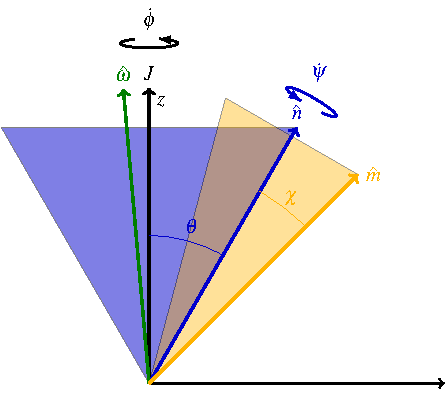
\includegraphics[width=0.33\textwidth]
    {/home/greg/Neutron_star_modelling/Illustrations/Cones/chi_less_theta.pdf}}
	\subfloat[$\theta = \chi$]{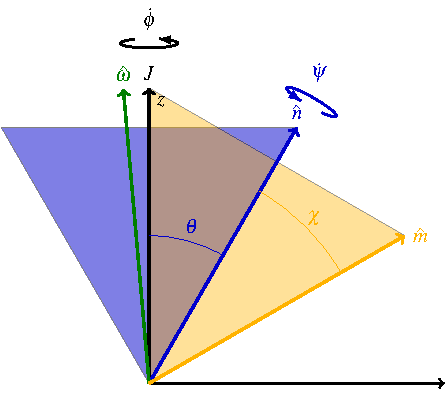
\includegraphics[width=0.33\textwidth]
    {/home/greg/Neutron_star_modelling/Illustrations/Cones/chi_equal_theta.pdf}}
	\subfloat[$\theta < \chi$]{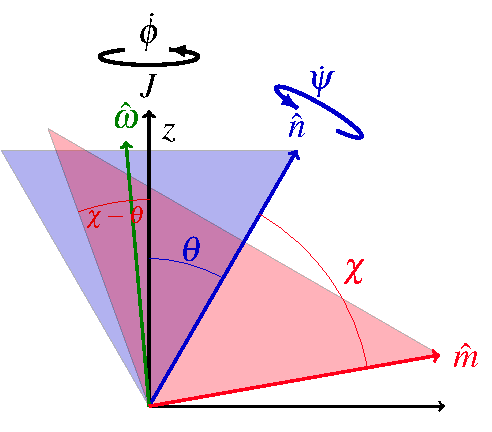
\includegraphics[width=0.33\textwidth]
    {/home/greg/Neutron_star_modelling/Illustrations/Cones/chi_more_theta.pdf}}
\caption{Diagrams depicting 2D projections of the cones swept out by the
    different motions under torque free precession onto the reference plane.
    The yellow cone is swept out by the rotation of $\m$ about $\n_{d}$ at the
    slow precession frequency; the blue cone is swept out by the rotation of
    $\n_{d}$ about $\J$ at the fast spin frequency. The
precession cone rotates in the opposing direction to the spin cone for oblate
bodies.}
\label{fig: cones}
\end{figure}

The motion of the magnetic dipole about the precession cone evolves on a much
longer timescale than its motion about the spin cone; as a result the star will
always pulsate once every spin period, but the long precession will modulate
the average value on the precession timescale. Because of the large difference
in timescales, the motion of $\m$ can be considered as the slow evolution of a
third cone swept out by $\m$ about $\J$ which we will call the dipole cone. The
half angle made by this cone is exactly the polar angle $\Theta$ calculated
in equation \eqref{eqn: Theta}. The frequency with which $\m$ rotates around
dipole cone is given by equation \eqref{eqn: Phi_dot}. In figures \ref{fig:
variations}(a) and (b) the polar angle and frequency modulations are plotted for
three particular cases, with reference to these plots we now discuss the three
cases:

\begin{itemize}
\item The $\chi = \theta/2$ case: the precession cone is narrow and does not
extend over the angular momentum vector. The polar angle $\Theta$ of the dipole
cone oscillates periodically between $\theta+\chi$ and $\theta-\chi$
during a precession cycle. The spin frequency $\dot{\Phi}$ has an average value
of $\dot{\phi}$ and
oscillates about this value, comparing with the $\Theta$ variations
demonstrates these oscillations are locked in phase with the rotation of $\m$
in the precession cone. Recalling that the precession cone counter rotates with
respect to the spin cone, at $\theta+\chi$ the precession cone motion acts in
the opposing direction to the spin cone, this causes a reduction in the spin
frequency away from the average; by contrast at $\theta+\chi$ the counter
rotation is now in favour of the spin frequency and as a result the spin
frequency is increased above the average.

\item The $\chi = \theta$ case: here the angular momentum vector sits exactly
on the side of the precession cone, this suggest $\m$ can align exactly with
the angular momentum. When this happens the spin frequency tends to zero (due
to numerical error, this never actually occurs) manifesting as sharp dips in the
spin frequency; at the same time the polar angle tends to zero.

\item The $\chi = 4\theta$ case: The precession cone now extends over the
angular momentum vector, this means it always acts to reduce the spin
frequency; as a result the spin frequency has an average value of
$\dot{\phi} + \dot{\psi}$. The polar angle can vary between $\theta+\chi$ and
$\chi-\theta$, for $\chi$ close to $\theta$ the deviations away from the
average are large while as $\chi$ increases the deviations get smaller as
the half angle of the dipole cone increases.
\end{itemize}•

\begin{figure}[ht]
\centering
	\subfloat[Variations in polar angle]
  {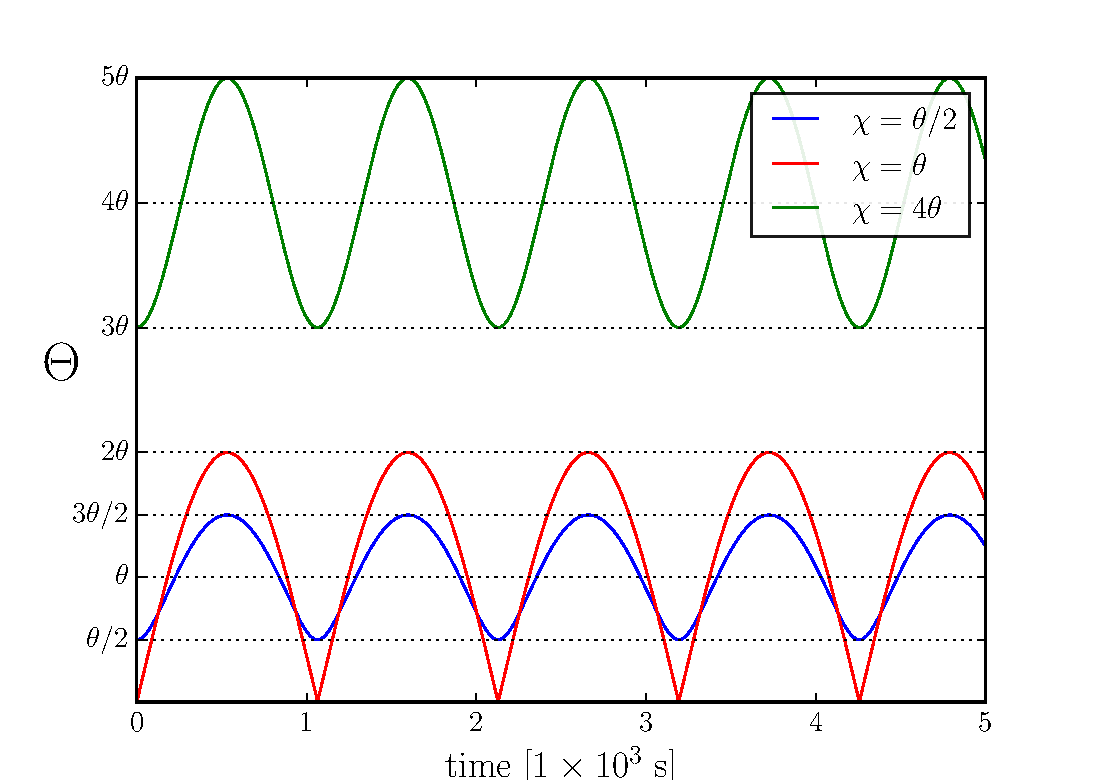
\includegraphics[width=0.7\textwidth]{polar_angle_variation_with_chi.pdf}}\\
	\subfloat[Variations in the spin frequency]
  {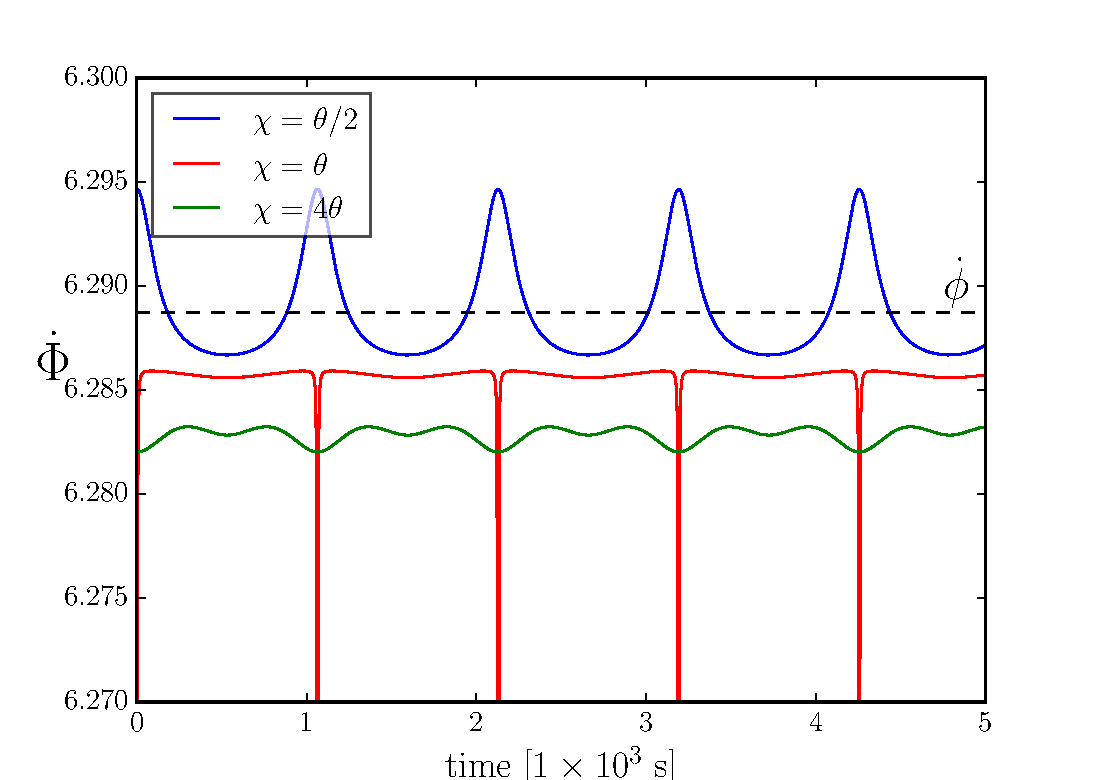
\includegraphics[width=0.7\textwidth]{frequency_variation_with_chi.pdf}} 
\caption{}
\label{fig: variations}
\end{figure}

\FloatBarrier
%\paragraph{Timing residuals}
%We now consider the timing residuals which would result from free precession
%alone. Clearly these are far from reality since the observed electromagnetic
%signal must act some torque on the body. Nevertheless, we can use equation
%\eqref{eqn: Phi} to calculate the exact phase of the signal. To compare with
%the tools used by observational astronomers we calculate the timing residual
%by fitting a third order Taylor series expansion to this phase. The residual
%is then the difference after subtraction
%
%\begin{figure}[ht]
%	\subfloat[$\chi<\theta$]{\includegraphics[width=0.5\textwidth]{{../../Timing_residuals/TR_chi_10.00}.png}}
%	\subfloat[$\chi > \theta$]{\includegraphics[width=0.5\textwidth]{{../../Timing_residuals/TR_chi_20.00}.png}}
%\caption{}
%\label{fig: }
%\end{figure}•

%\subsection{Biaxial body with torque}
%We now introduce the torque using the parameters of pulsar B1828-11 (Need to
%reference values here) to simulate a realistic pulsar making some assumptions
%on the cause of the periodic modulations. With realistic values the spin
%period is approximately a second, in comparison the precession period of the
%order of a year. The result is that we must resolve $10^{7}$ rotations of the
%neutron star per precessional orbit. 
%
%\begin{figure}[ht]
%	\subfloat[]{\includegraphics[width=0.5\textwidth]{{Spherical_Plot_chi_70.0_epsI1_0.00e+00_epsI3_9.37e-09_epsA_6.94e-12_omega0_15.51_aint_15_t1_3.00e+08}.pdf}}
%	\subfloat[]{\includegraphics[width=0.5\textwidth]{{Euler_Angles_chi_70.0_epsI1_0.00e+00_epsI3_9.37e-09_epsA_6.94e-12_omega0_15.51_aint_15_t1_3.00e+08}.pdf}}
%\caption{}
%\label{fig: }
%\end{figure}

\FloatBarrier

%\biblio
\end{document}

